\textbf{COLUNI 2025 -- Questão 23}\par\medskip As figuras abaixo representam circuitos elétricos constituídos de fios condutores de resistência elétrica, praticamente desprezível, uma bateria e lâmpadas $L_1$, $L_2$, $L_3$, $L_4$, $L_5$ e $L_6$, de resistências elétricas $R$ idênticas. Sabe-se que, para o funcionamento do circuito, há a necessidade da existência de uma diferença de potencial, fornecida pela bateria, nos terminais do mesmo, e que o brilho das lâmpadas está diretamente relacionado à intensidade da corrente elétrica que as atravessam. Quando um caminho de resistência elétrica desprezível liga os polos positivos e negativos da fonte de energia, a corrente elétrica passará toda por ele e ocorrerá curto-circuito.

\begin{center}Circuito I\hfill Circuito II\hfill Circuito III\end{center}

% COLUNI-AUTO-FIGURES-BEGIN
\begin{figure}[htbp]
\centering
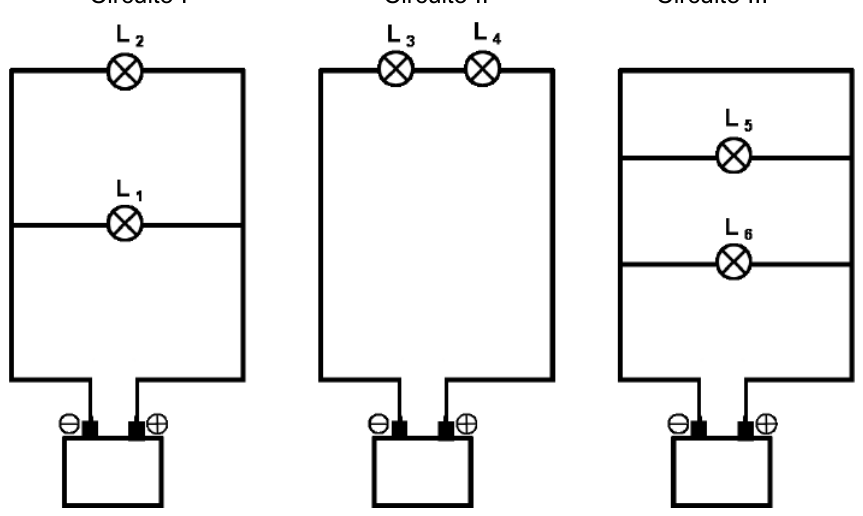
\includegraphics[width=0.95\linewidth]{static/simulados/coluni/figuras/2025/questao-23/figura-1.png}
\end{figure}
% COLUNI-AUTO-FIGURES-END

Considere as afirmações sobre os circuitos.
\begin{enumerate}
\item[I.] O brilho das lâmpadas do circuito I é o mesmo ao observado nas lâmpadas do circuito II.
\item[II.] O brilho das lâmpadas do circuito I é o mesmo ao observado nas lâmpadas do circuito III.
\item[III.] As lâmpadas do circuito II e do circuito III acendem e têm mesmo brilho.
\item[IV.] No circuito III, as lâmpadas não acendem e há curto-circuito.
\end{enumerate}
Está CORRETO o que se afirma apenas em:
\begin{enumerate}
\item I e IV.
\item II e III.
\item III.
\item IV.
\end{enumerate}
